\section*{ĐỀ TRẮC NGHIỆM CUỐI CHƯƠNG}
\Opensolutionfile{ans}[ans/ansTL-0H3-3]
\setcounter{ex}{0}
\subsubsection{Đề số 1}

\begin{ex}%[Bùi Sang Thọ]%[0H2B1]
	Tìm mệnh đề \textbf{sai} trong các mệnh đề sau:
	\choice
	{$\cos 0^\circ=1$}
	{$\sin 0^\circ=0$}
	{\True $\cos 120^\circ=\dfrac{2}{\sqrt{2}}$}
	{$\sin 120^\circ=\dfrac{\sqrt{3}}{2}$}
\end{ex}

\begin{ex}%[Bùi Sang Thọ]%[0H2B1]
	Tìm mệnh đề đúng trong các mệnh đề sau:
	\choice
	{$\sin 60^\circ=\dfrac{\sqrt{2}}{2}$}
	{$\tan 30^\circ=\sqrt{3}$}
	{$\cot 90^\circ=1$}
	{\True $\sin 135^\circ=\dfrac{\sqrt{2}}{2}$}
\end{ex}

\begin{ex}%[Bùi Sang Thọ]%[0H2B1]
	Cho $\alpha$ là góc tù. Mệnh đề nào đúng trong các mệnh đề sau?
	\choice
	{$\sin\alpha<0$}
	{$\cos\alpha>0$}
	{\True $\tan\alpha<0$}
	{$\cot\alpha>0$}
\end{ex}

\begin{ex}%[Bùi Sang Thọ]%[0H2B1]
	Tìm mệnh đề đúng trong các mệnh đề sau:
	\choice
	{\True $\sin\alpha=\sin(180^\circ-\alpha)$}
	{$\cos\alpha=\cos(180^\circ-\alpha)$}
	{$\tan\alpha=\tan(180^\circ-\alpha)$}
	{$\cot\alpha=\cot(180^\circ-\alpha)$}
\end{ex}

\begin{ex}%[Võ Thị Quỳnh Trang]%[0H2B1]
	Biết $\sin \alpha = \dfrac{1}{3}$. Tính $P= \cos^2 \alpha + 3\tan^2 \alpha$.
	\choice
	{\True $\dfrac{91}{72}$}
	{$\dfrac{5}{6}$}
	{$\dfrac{8}{9}$}
	{$\dfrac{67}{72}$}
\end{ex}

\begin{ex}%[Võ Thị Quỳnh Trang]%[0H2B1]
	\immini[thm]{Trên nửa đường tròn đơn vị, vị trí nào trong các vị trí dưới đây xác định điểm $M$ sao cho $\tan \widehat {xOM} = 1.$
		\haicot
		{\True Vị trí $(1)$}
		{Vị trí $(2)$}
		{Vị trí $(3)$}
		{Vị trí $(4)$}
	}
	{
		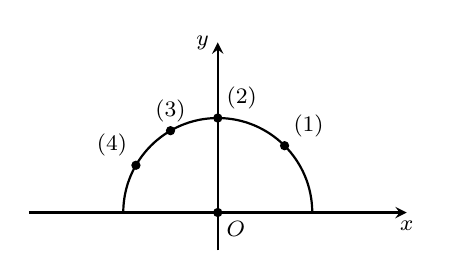
\begin{tikzpicture}[>=stealth,x=1.0cm,y=1.0cm,thick,scale=1.2]
			\begin{footnotesize}
				\draw[->] (-2,0) -- (2,0) node[below] {$x$};
				\draw[->] (0,-0.4) -- (0,1.8) node[left] {$y$};
				\coordinate (O) at (0,0);
				\fill[black] (0,0) circle[radius=1.4pt] node[below right]{\footnotesize $O$};
				\coordinate (M) at (0.7071,0.7071);
				\fill[black] (0.7071,0.7071) circle[radius=1.4pt] node[above right]{\footnotesize $(1)$};
				\draw (1,0) arc (0:180:1);
				\coordinate (P) at (-0.866,0.5);
				\fill[black] (-0.866,0.5) circle[radius=1.4pt] node[above left]{\footnotesize $(4)$};
				\coordinate (N) at (-0.5,0.866);
				\fill[black] (-0.5,0.866) circle[radius=1.4pt] node[above ]{\footnotesize $(3)$};
				\coordinate (Q) at (0,1);
				\fill[black] (0,1) circle[radius=1.4pt] node[above right]{\footnotesize $(2)$};
				
			\end{footnotesize}
		\end{tikzpicture}
	}	
\end{ex}

\begin{ex}%[Dương BùiĐức,Đề thi HKI khối 10 năm học 2019-2020]%[0H2B3-4]%
	Cho tam giác $ABC$ có độ dài các cạnh $AB=5$, $AC=8$, $BC=7$. Tính số đo góc $A$.
	\choice
	{$120^{\circ}$}
	{\True $60^{\circ}$}
	{$45^{\circ}$}
	{$30^{\circ}$}
	\loigiai{
		Ta có
		$$\cos A = \dfrac{b^2 + c^2 - a^2}{2bc} = \dfrac{64 + 25 - 49}{2.40} = \dfrac{1}{2} \Rightarrow A = 60^\circ.$$}
\end{ex}

\begin{ex}%[0H2B3]
	Cho tam giác $ABC$ có $AB=3,$ $BC=4,$ $AC=5.$ Độ dài đoạn trung tuyến $AM$ là
	\choice
	{$13$}
	{\True $\sqrt{13}$}
	{$\dfrac{\sqrt{26}}{2}$}
	{$\dfrac{13}{2}$}
\end{ex}

\begin{ex}%[Trần Minh,Chuyển sách Tex - 10, 11 (dự án 3)]%[0H2B3-1]
	Tam giác $ ABC$ cân tại $ C$, có $ AB=9$ cm và $ AC=\dfrac{15}{2}$ cm. Gọi $ D$ là điểm đối xứng của $ B$ qua $ C$. Tính độ dài cạnh $ AD$ 
	\choice
	{$ AD=6$ cm}
	{$ AD=9$ cm}
	{\True $ AD=12$ cm}
	{$ AD=12\sqrt{2}$ cm}
	\loigiai{
		\immini{
			Ta có $ D$ là điểm đối xứng của $ B$ qua $ C$ suy ra $ C$ là trung điểm của $ BD$. \\
			$ \Rightarrow  AC$ là trung tuyến của tam giác $DAB$. \\
			Suy ra $ BD=2BC=2AC=15$. \\
			Theo hệ thức trung tuyến ta có\\
			$\begin{aligned}
				&AC^2=\dfrac{AB^2+AD^2}{2}-\dfrac{BD^2}{4}\\ \Rightarrow& AD^2=2AC^2+\dfrac{BD^2}{2}-AB^2\\
				\Rightarrow& AD^2= 2\cdot \left(\dfrac{15}{2} \right)^2+\dfrac{15^2}{2}-9^2=144.\\
				\Rightarrow &AD=12.
			\end{aligned}$ 
		}
		{\begin{tikzpicture}[scale=1,font=\footnotesize,line join=round, line cap=round,>=stealth]
				\tkzDefPoints{0/0/A,0/4/D,3/0/B}
				\tkzDefMidPoint(D,B) \tkzGetPoint{C}
				\tkzDrawPoints[fill=black](A,B,C,D)
				\tkzDrawPolygon(A,B,D)
				\tkzDrawSegments(A,C)
				\tkzLabelPoints[above](D) 
				\tkzLabelPoints[below](B,A)
				\tkzLabelPoints[right](C) 
				\tkzMarkRightAngles[size=0.2](D,A,B)
		\end{tikzpicture}}
	}
\end{ex}

\begin{ex}%[Trần Minh,Chuyển sách Tex - 10, 11 (dự án 3)]%[0H2Y3-1]
	Tam giác $ ABC$ có $ BC=10$ và $ \widehat{A}=30^\circ$. Tính bán kính $ R$ của đường tròn ngoại tiếp tam giác $ ABC$.
	\choice
	{$ R=5$}
	{\True $ R=10$}
	{$ R=\dfrac{10}{\sqrt{3}}$}
	{$ R=10\sqrt{3}$}
	\loigiai
	{Áp dụng định lí sin, ta có $ \dfrac{BC}{\sin A}=2R\Rightarrow R=\dfrac{BC}{2}\cdot \sin  A=\dfrac{10}{2}\cdot \sin 30^\circ=10$.}
\end{ex}

\begin{ex}%[Trần Minh,Chuyển sách Tex - 10, 11 (dự án 3)]%[0H2Y3-1]
	Tam giác $ ABC$ có $ AB=3$, $AC=6$, $\widehat{BAC}=60^\circ $. Tính diện tích tam giác $ ABC$.
	\choice
	{$ S_{\Delta ABC}=9\sqrt{3}$}
	{\True $ S_{\Delta ABC}=\dfrac{9\sqrt{3}}{2}$}
	{$ S_{\Delta ABC}=9$}
	{$ S_{\Delta ABC}=\dfrac{9}{2}$}
	\loigiai
	{Ta có $ S_{\Delta ABC}=\dfrac{1}{2}\cdot AB\cdot AC\cdot \sin{A}=\dfrac{1}{2}\cdot 3\cdot 6\cdot \sin 60^\circ=\dfrac{9\sqrt{3}}{2}$.}
\end{ex}
\begin{ex}%[Trần Minh,Chuyển sách Tex - 10, 11 (dự án 3)]%[0H2Y3-1]
	Tam giác $ ABC$ có $ AC=4$, $\widehat{BAC}=30^\circ$, $\widehat{ACB}=75^\circ $. Tính diện tích tam giác $ ABC$.
	\choice
	{$ S_{\Delta ABC}=8$}
	{$ S_{\Delta ABC}=4\sqrt{3}$}
	{\True $ S_{\Delta ABC}=4$}
	{$ S_{\Delta ABC}=8\sqrt{3}$}
	\loigiai
	{Ta có $ \widehat{ABC}=180^\circ-(\widehat{BAC}+\widehat{ACB} )=75^\circ =\widehat{ACB}$.\\
		Suy ra tam giác $ ABC$ cân tại $ A$ nên $ AB=AC=4$.\\
		Diện tích tam giác $ ABC$ là $ S_{\Delta ABC}=\dfrac{1}{2}AB\cdot AC\sin \widehat{BAC}=4$.}
\end{ex}
\begin{ex}%[Trần Minh,Chuyển sách Tex - 10, 11 (dự án 3)]%[0H2B3-1]
	Tam giác $ ABC$ có $ a=21$, $b=17$, $c=10$. Diện tích của tam giác $ ABC$ bằng
	\choice
	{$ S_{\Delta ABC}=16$}
	{$ S_{\Delta ABC}=48$}
	{$ S_{\Delta ABC}=24$}
	{\True $ S_{\Delta ABC}=84$}
	\loigiai
	{Ta có $ p=\dfrac{21+17+10}{2}=24$.\\
		Do đó $ S=\sqrt{p(p-a )(p-b )(p-c )}=\sqrt{24(24-21 )(24-17 )(24-10 )}=84$.}
\end{ex}

\begin{ex}%[Trần Minh,Chuyển sách Tex - 10, 11 (dự án 3)]%[0H2B3-1]
	Tam giác $ ABC$ có $ AB=5$, $AC=8$ và $ \widehat{BAC}=60^\circ$. Tính bán kính $ r$ của đường tròn nội tiếp tam giác đã cho.
	\choice
	{$ r=1$}
	{$ r=2$}
	{\True $ r=\sqrt{3}$}
	{$ r=2\sqrt{3}$}
	\loigiai
	{Áp dụng định lý hàm số cô-sin, ta có
		$ BC^2=AB^2+AC^2-2AB\cdot AC\cos A=49\Rightarrow BC=7$.\\
		Diện tích $ S=\dfrac{1}{2}AB\cdot AC\cdot \sin A=\dfrac{1}{2}\cdot 5\cdot 8\cdot \dfrac{\sqrt{3}}{2}=10\sqrt{3}$.\\
		Lại có $ S=p\cdot r\Rightarrow r=\dfrac{S}{p}=\dfrac{2S}{AB+BC+CA}=\sqrt{3}$.}
\end{ex}
\begin{ex}%[Trần Minh,Chuyển sách Tex - 10, 11 (dự án 3)]%[0H2B3-1]
	Tam giác $ ABC$ có $ a=21$, $b=17$, $c=10$. Tính bán kính $ r$ của đường tròn nội tiếp tam giác đã cho.
	\choice
	{$ r=16$}
	{$ r=7$}
	{\True $ r=\dfrac{7}{2}$}
	{$ r=8$}
	\loigiai
	{Ta có $ p=\dfrac{21+17+10}{2}=24$.\\
		Suy ra $ S=\sqrt{24(24-21 )(24-17 )(24-10 )}=84$.\\
		Lại có $ S=p\cdot r\Rightarrow r=\dfrac{S}{p}=\dfrac{84}{24}=\dfrac{7}{2}$.}
\end{ex}

\begin{ex}%[0H2K3-4]%
	Cho hình chữ nhật ${ABCD}$ có cạnh $AB=4$, $BC=6$, $M$ là trung điểm của ${BC}$, $N$ là điểm trên cạnh ${CD}$ sao cho ${ND = 3NC}$ . Khi đó bán kính của đường tròn ngoại tiếp tam giác ${AMN}$ bằng
	\choice
	{$5\sqrt{2}$ }
	{$3\sqrt{5}$ }
	{\True $\dfrac{5\sqrt{2}}{2}$ }
	{$\dfrac{3\sqrt{5}}{2}$ }
	\loigiai{
		\immini{Ta có: \\
			$ MC=3$, $NC=1\Rightarrow MN=\sqrt{10}$,
			$ BM=3$, $AB=4\Rightarrow AM=5$,  \\
			$ AD=6$, $ND=3\Rightarrow AN=\sqrt{45}$,   \\
			$ p=\dfrac{AM+AN+MN}{2}=\dfrac{\sqrt{10}+5+\sqrt{45}}{2}$, \\
			$ {{S}_{AMN}}=\sqrt{p\left( p-AM \right)\left( p-AN \right)\left( p-MN \right)}=\dfrac{15}{2}$ \\
			Bán kính của đường tròn ngoại tiếp của tam giác $AMN$ là:\\ $R=\dfrac{AM.AN.MN}{4{{S}_{AMN}}}=\dfrac{5\sqrt{2}}{2}$
		}{\begin{tikzpicture}[line join = round]
				\draw(-3,-2)coordinate(A)--(-3,2)coordinate(B)--(3,2)coordinate(C)--(3,-2)coordinate(D)--cycle;
				\draw(A)--($(B)!.5!(C)$)coordinate(M)--($(C)!1/3!(D)$)coordinate(N)--cycle;
				\foreach \p/\g in {A/-135,B/135,C/45,D/-45,M/90,N/0}\draw[fill=white](\p)circle (1pt)node [shift={(\g:.25)}] {$\p$};
				%\draw[gray,ultra thin](-3,-3)grid(3,3);
		\end{tikzpicture}}
	}
\end{ex}

\begin{ex}%[Trần Minh,Chuyển sách Tex - 10, 11 (dự án 3)]%[0H2B3-4]
	\immini[thm]{
		Xác định chiều cao của một tháp mà không cần lên đỉnh của tháp. Đặt kế giác thẳng đứng cách chân tháp một khoảng $ CD=60$ m, giả sử chiều cao của giác kế là $ OC=1$ m. Quay thanh giác kế sao cho khi ngắm theo thanh ta nhình thấy đỉnh $ A$ của tháp. Đọc trên giác kế số đo của góc $ \widehat{AOB}=60^\circ$. Chiều cao của ngọn tháp gần với giá trị nào sau đây:
		\choicew{0.5\textwidth}
		\choice
		{$ 40$ m}
		{ $ 114$ m} 
		{ \True $ 105$ m} 
		{ $ 110$ m}
	}
	{
		\begin{tikzpicture}[scale=0.7, font=\footnotesize, line join = round, line cap = round,>=stealth]
			\tkzDefPoints{0/2.5/O',0/6.5/I,0/1.75/B,6/1.75/O,0/9/A,0/0/D,6/0/C}
			\draw [line width=3, brown
			] (-1.2,0.1)--(-0.26,2) (-0.24,-0.2)--(-0.13,2) (0.32,0.3)--(0.08,2) (1,0.1)--(0.24,2.06) (0,6.8)--(0,7.7);
			\draw [line width=5, brown
			]  (-0.2,3.28)--(-0.16,6.24) (0.2,3.28)--(0.16,6.24)  (-0.1,3.5)--(0.1,3.5) (-0.1,4)--(0.1,4) (-0.1,4.5)--(0.1,4.5) (-0.1,5)--(0.1,5) (-0.1,5.5)--(0.1,5.5)  (-0.1,6)--(0.1,6);
			\draw [line width=2, brown
			]  (0,7.7)--(0,9) ;
			\tkzDrawArc[R,fill=yellow](O',0.75cm)(0,360)
			\tkzDrawArc[R,fill=yellow](I,0.4cm)(0,360)
			\tkzDrawArc[R](O,0.75cm)(0,360)
			\tkzDrawPoints[fill=black](A,B,C,D,O)
			\tkzDrawSegments(O,C)
			\tkzDrawLines[add = 0 and 0.05](A,O B,O)
			\tkzDrawLines[add = 0.3 and 0.05](D,C)
			\tkzLabelPoints[above](A,O)  
			\tkzLabelPoints[below](D,C)
			\tkzLabelPoints[above](B)
			\tkzLabelAngles[pos=0.5](A,O,B){$60^{\circ}$}
		\end{tikzpicture}
	}
	\loigiai
	{Tam giác $ OAB$ vuông tại $ B$, có $ \tan \widehat{AOB}=\dfrac{AB}{OB}\Rightarrow AB=\tan 60^\circ\cdot OB=60\sqrt{3}$ m. \\
		Vậy chiếu cao của ngọn tháp là $ h=AB+OC=(60\sqrt{3}+1)\simeq 105$ m.}
\end{ex}
\begin{ex}%[Trần Minh,Chuyển sách Tex - 10, 11 (dự án 3)]%[0H2B3-4]
	\immini[thm]
	{
		Từ hai vị trí $ A$ và $ B$ của một tòa nhà, người ta quan sát đỉnh $ C$ của ngọn núi. Biết rằng độ cao $ AB=70$ m, phương nhìn $ AC$ tạo với phương nằm ngang góc $ 30^\circ$, phương nhìn $ BC$ tạo với phương nằm ngang góc $ 15^\circ30'$. Ngọn núi đó có độ cao so với mặt đất gần nhất với giá trị nào sau đây?
		\choicew{0.5\textwidth}
		\choice
		{\True $ 135$ m}
		{$ 234$ m} { $ 165$ m}
		{$ 195$ m}
	}
	{
		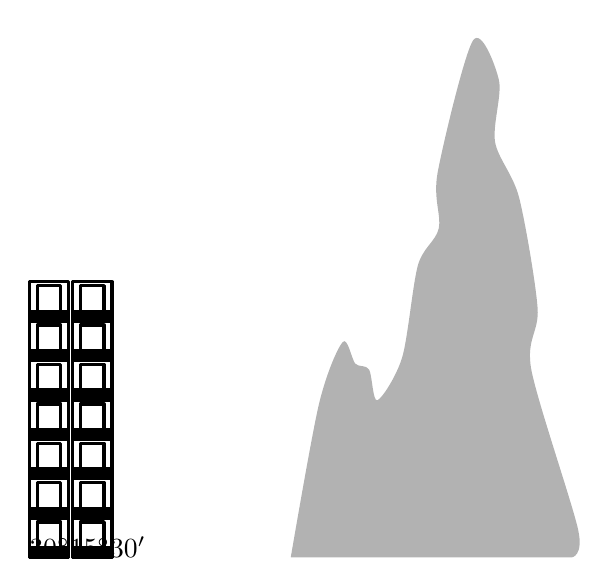
\begin{tikzpicture}[scale=.5, font=\footnotesize, line join=round, >=stealth]
			\tkzDefPoints{0/0/O,2.2/0/A,2.2/7/B,11.27/13.13/C,11.27/7/D,14/0/E}
			\tkzDrawSegments(C,B C,A A,E)
			\tkzDrawSegments[dashed](B,D)
			\def\nhathap{6} %so tang nha thap
			\def\dai{1} %chieu dai 1 khoi
			\def\cao{1} %chieu cao 1 khoi
			\newcommand{\xaynha}[2]{
				\draw[very thick] (#1,#2)rectangle(#1+\dai,#2+\cao);
				\draw[very thick,fill=black] (#1,#2)rectangle(#1+\dai,#2+0.25*\cao);
				\draw[very thick] (#1+0.2*\dai,#2+0.25*\cao)rectangle(#1+0.8*\dai,#2+0.9*\cao); 
			}
			%Xay nha thap
			\foreach \j in {0,...,\nhathap}{
				\foreach \i in {0,1}{
					\xaynha{\i*1.1}{\j*\cao}
				} 
			}
			\tkzLabelPoints[above](C,B) 
			\tkzLabelPoints[below](A)
			\fill [black!30]plot [smooth ] coordinates{(6.64,0)(7.36,3.91) (7.96,5.47) (8.28,4.92) (8.63,4.77)(8.84,3.99) (9.47,5.08) (9.87,7.42)(10.4,8.36)(10.37,9.77)(11.27,13.13)(11.93,12.11)(11.83,10.55)(12.44,9.14)(12.91,6.33)(12.75,4.77)(13.94,0.7)(13.78,0)};
			%\tkzMarkAngles[size=1cm,arc=ll,mark=|](E,A,C)
			%\tkzMarkAngles[size=1cm,arc=l,mark=||](D,B,C)
			\tkzLabelAngles[right,pos=1](E,A,C){$30^\circ$}
			\tkzLabelAngles[right,pos=1](D,B,C){$15^\circ30'$}
			\tkzDrawArc[R](A,1cm)(0,54)
			\tkzDrawArc[R](B,1cm)(0,37)
			\tkzDrawArc[R](B,0.9cm)(0,37)
		\end{tikzpicture}
	}
	
	\loigiai
	{Từ giả thiết, ta suy ra tam giác $ ABC$ có $ \widehat{CAB}=60^\circ$, $\widehat{ABC}=105^\circ30'$ và $ AB=70$. \\
		Khi đó $ \widehat{A}+\widehat{B}+\widehat{C}=180^\circ\Leftrightarrow \widehat{C}=180^\circ-(\widehat{A}+\widehat{B} )=180^\circ-165^\circ30'=14^\circ30'$. \\
		Theo định lí sin, ta có $ \dfrac{AC}{\sin B}=\dfrac{AB}{\sin C}\Rightarrow AC=\dfrac{70\cdot \sin 105^\circ30'}{\sin 14^\circ30'}\simeq  269{,}4$ m. \\
		Gọi $ CH$ là khoảng cách từ $ C$ đến mặt đất. \\
		Tam giác vuông $ ACH$ có cạnh $ CH$ đối diện với góc $ 30^\circ$ nên $ CH=\dfrac{AC}{2}=\dfrac{269,4}{2}=134{,}7$ m. \\
		Vậy ngọn núi cao khoảng $ 135$ m.}
\end{ex}

\begin{ex}%[WTT-1234 câu TN10, Trần Minh]%[0H2B3-4]%
	\immini[thm]{Khoảng cách từ $A$ đến $B$ không thể đo trực tiếp được vì phải qua một đầm lầy. Người ta xác định được một điểm $C$ mà từ đó có thể nhìn được $A$ và $B$ dưới một góc $60^{\circ}$. Biết $CA=200$ m, $CB=180$ m. Khoảng cách $AB$ bằng bao nhiêu?
	\haicot
	{\True $20\sqrt{91}$ m}
	{$112$ m}
	{$168$ m}
	{$228$ m}}{
	\begin{tikzpicture}[scale=1, font=\footnotesize, line join = round, line cap = round]
		\tkzDefPoints{0/0/A,5/0/B,2/3/C,1/0/M,4/0/N}
		\tkzDrawPoints[](A,B,C)
		\tkzDrawSegments(C,A C,B A,M N,B)
		\tkzLabelPoints[below](A,B)
		\tkzLabelPoints[above](C)
		\draw plot [smooth cycle] coordinates{(1,0)(1.5,1.2) (2,1) (3,1.5) (4,0)(3,-1.2) (2.5,-0.75) (2,-1)};
		\fill[pattern=north east lines,opacity=0.5] plot [smooth cycle] coordinates{(1,0)(1.5,1.2) (2,1) (3,1.5) (4,0)(3,-1.2) (2.5,-0.75) (2,-1)};
\end{tikzpicture}}
	\loigiai{
		\immini
		{Ta có\\
			$\begin{aligned}
				AB^2&=CA^2+CB^2-2\cdot CA\cdot CB\cdot \cos 60^{\circ}\\
				&=36400.
			\end{aligned}$\\
			$ \Rightarrow AB=20\sqrt{91}$ m.}
		{
			\begin{tikzpicture}[scale=1, font=\footnotesize, line join = round, line cap = round]
				\tkzDefPoints{0/0/A,5/0/B,2/3/C,1/0/M,4/0/N}
				\tkzDrawPoints[](A,B,C)
				\tkzDrawSegments(C,A C,B A,M N,B)
				\tkzLabelPoints[below](A,B)
				\tkzLabelPoints[above](C)
				\draw plot [smooth cycle] coordinates{(1,0)(1.5,1.2) (2,1) (3,1.5) (4,0)(3,-1.2) (2.5,-0.75) (2,-1)};
				\fill[pattern=north east lines,opacity=0.5] plot [smooth cycle] coordinates{(1,0)(1.5,1.2) (2,1) (3,1.5) (4,0)(3,-1.2) (2.5,-0.75) (2,-1)};
			\end{tikzpicture}
	}}
\end{ex}

\begin{ex}%[0H2G3-4]%
	\immini[thm]
	{Vòng quay mặt trời Hạ Long Sun Wheel trong khu giải trí Sun World Ha Long Park có đường kính $115m$, quay hết một vòng trong thời gian $20$ phút. Lúc bắt đầu quay, một người ở cabin thấp nhất cách mực nước biển $100m$. Hỏi người đó đạt được độ cao $200m$ (so với mực nước biển) lần đầu tiên sau bao nhiêu giây (làm tròn đến $1/10$ giây)?
		\haicot
		{$460,6$ giây}
		{$407,9$ giây}
		{$408,6$ giây}
		{\True $458,9$ giây}
	}
	{
		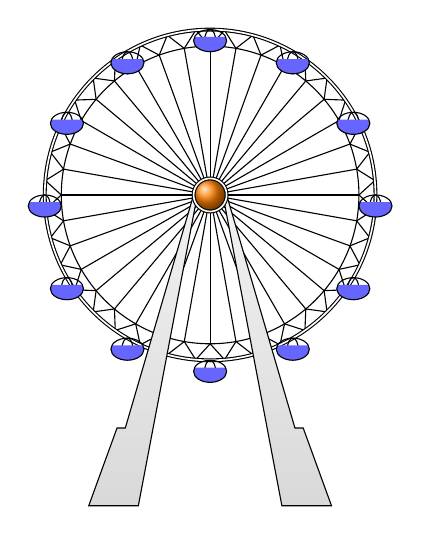
\begin{tikzpicture}[scale=0.7]
			\def\r{3}
			\def\a{\r/10}
			\def\n{36}%Số nan đu quay
			\def\m{12}%Số lồng đu quay
			\pgfmathsetmacro{\g}{20}
			\pgfmathsetmacro{\b}{2*\a/3}
			\pgfmathsetmacro{\xo}{\a *cos(\g)}
			\pgfmathsetmacro{\yo}{\b *sin(\g)}
			\def\longdq(#1:#2){
				\begin{scope}[shift={(#1:#2)}]
					\draw (0,-\b) ellipse ({\b/2} and {\b});
					\fill[blue!60] (\xo,\yo-\b) arc (\g:-180-\g:{\a} and {\b})--cycle;
					\draw (0,-\b) ellipse({\a} and {\b});
				\end{scope}
			}
			\foreach \i in {1,...,\n}{
				\pgfmathsetmacro{\gm}{360*\i/\n}
				\pgfmathsetmacro{\gh}{(360*\i+180)/\n}
				\pgfmathsetmacro{\gb}{360*(\i+1)/\n}
				\draw (\gm:\r-\a)--(\gh:\r)--(\gb:\r-\a);
				\draw (\gm:\r-\a)--(\gm:\a);
			}
			\draw[double] (0:0) circle (\r);
			\draw (0:0) circle (\r-\a);
			\foreach \i in {1,...,\m}{\longdq(360*\i/\m:\r)}
			\draw[top color =gray!10, bottom color=gray!30] (-30:\a) arc(-30:0:\a) --(-70:1.5*\r)--++(\a/2,0)--([turn]-70:\r/2) --([turn]-110:3*\a)--(-30:\a);
			\draw[top color =gray!10, bottom color=gray!30, xscale=-1] (-30:\a) arc(-30:0:\a) --(-70:1.5*\r)--++(\a/2,0)--([turn]-70:\r/2) --([turn]-110:3*\a)--(-30:\a);
			\fill[ball color=orange] (0:0) circle (\a);
			\draw[double] (0:0) circle (\a);
		\end{tikzpicture}
	}
	\loigiai
	{
		\immini
		{
			$OA=\dfrac{115}{2}m$; $OH=100-OA=\dfrac{85}{2}m$.\\
			$\cos \alpha =\dfrac{OH}{OB}=\dfrac{\dfrac{85}{2}}{\dfrac{115}{2}}=\dfrac{17}{23} \Rightarrow \Delta \varphi =\pi -\alpha \approx 0,765\pi $.\\
			$t=\dfrac{\Delta \varphi}{\omega}$ với $\omega $ là tốc độ góc.\\ $T=\dfrac{2\pi}{\omega}$ với $T$ là chu kì.\\
			$T=20$ phút $=20 \cdot 60=1200$ giây.\\
			$ \Rightarrow \omega =\dfrac{2\pi}{T}=\dfrac{2\pi}{1200}=\dfrac{\pi}{600} \Rightarrow t \approx \dfrac{0,765\pi}{\dfrac{\pi}{600}} \approx 459$ giây.
		}
		{
			\begin{tikzpicture}
				\coordinate (O) at (0,0);
				\coordinate (A) at (0,-3);
				\coordinate (K) at (3,0);
				\coordinate (C) at (0,3);
				\coordinate (H) at (0,1.5);
				\draw let \p1=($(K)-(O)$) in (O) circle ({veclen(\x1,\y1)}); % Vẽ đường tròn tâm O đi qua điểm A
				\coordinate (B) at ($(O)!1!30:(K)$); % Quay hướng 60 độ và vị tự tỉ số 1 điểm B tâm A thành điểm B1
				\fill[black] (A)node[below]{$A$} circle (1.5pt);
				\fill[black] (O)node[left]{$O$} circle (1.5pt);
				\fill[black] (H)node[left]{$H$} circle (1.5pt);
				\fill[black] (B)node[right]{$B$} circle (1.5pt);
				\draw[line width=0.4pt,black] (A)--(C) (B)--(H) (O)--(B); % Đoạn thẳng AB
				\draw pic[draw,blue,angle radius=5mm,angle eccentricity=1.5,"$\alpha$"] {angle = B--O--H}; % Vẽ góc BAC với tên nhãn \beta. Nếu vẽ góc vuông thì thay angle = thành right angle =
				\draw pic[draw,red,angle radius=3mm,angle eccentricity=2.5,"$\Delta \varphi$"] {angle = A--O--B};
			\end{tikzpicture}
		}
	}
\end{ex}
\centerline{\textbf{---HẾT---}}
\Closesolutionfile{ans}
